\documentclass[11pt,letterpaper]{article}
\usepackage[utf8]{inputenc}
\usepackage{amsmath,amssymb,fullpage,graphicx}
\usepackage{afterpage}

\begin{document}
\subsection*{Lect 18-3}
\subsection*{a}
\begin{verbatim}
design1 <- gen.factorial(c(2,2,2), varNames = c('A','B','C'))
attach(design1)
A <- as.factor(A)
B <- as.factor(B)
C <- as.factor(C)
y <- c(22, 32, 35, 55, 44, 40, 60, 39)

contr <- as.character("contr.helmert")
lm1 <- lm(y~A*B*C, contrasts = list(A=contr,B=contr,C=contr))

summary.aov(lm1)
            Df Sum Sq Mean Sq
A            1    3.1     3.1
B            1  325.1   325.1
C            1  190.1   190.1
A:B          1    6.1     6.1
A:C          1  378.1   378.1
B:C          1   55.1    55.1
A:B:C        1   91.1    91.1

eff1 <- 2 * (lm1$coefficients)[-1]
qqnorm(eff1)
abline(median(eff1), 7)
\end{verbatim}

\noindent From the ANOVA table, we can perceive the residual is zero, since there is no replication, number of parameter is over number of runs. 

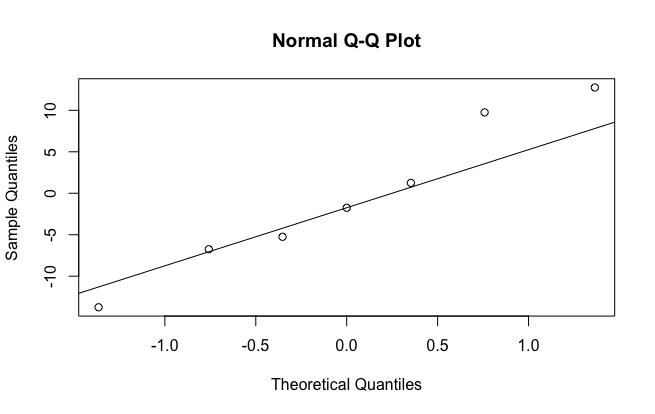
\includegraphics[scale=0.55]{lect18-3-a.png}

\subsection*{b}
\noindent From the qqplot, we can see factors with lowest effect and two highest effect are excluded from pattern of a line. They are factors of B, C and AC. Due to principle of hierarchy, factor A should also be included in new model. 

\begin{verbatim}
lm2 <- lm(y~A+B+C+A:C)
summary.aov(lm2)
            Df Sum Sq Mean Sq F value Pr(>F)  
A            1    3.1     3.1   0.062 0.8201  
B            1  325.1   325.1   6.401 0.0854 .
C            1  190.1   190.1   3.743 0.1485  
A:C          1  378.1   378.1   7.445 0.0720 .
Residuals    3  152.4    50.8 
\end{verbatim}

\subsection*{c}
\begin{verbatim}
rm(list=ls(all=T))
y <- c(22, 32, 35, 55, 44, 40, 60, 39)
design2 <- gen.factorial(c(2,2,2), varNames = c('A','B','C'))
attach(design2)
ABC <- A*B*C
A <- as.factor(A)
B <- as.factor(B)
C <- as.factor(C)
Block <- as.factor(ABC)
contr <- as.character("contr.helmert")
lm3 <- lm(y~A*B*C + Block, contrasts = list(A=contr,B=contr,C=contr, Block=contr))

summary.aov(lm3)
            Df Sum Sq Mean Sq
A            1    3.1     3.1
B            1  325.1   325.1
C            1  190.1   190.1
Block        1   91.1    91.1
A:B          1    6.1     6.1
A:C          1  378.1   378.1
B:C          1   55.1    55.1
\end{verbatim}

\noindent Since ABC effect is confounded with block effect, ABC effect is not shown on the ANOVA table. 

\subsection*{d}
\begin{verbatim}
contr <- as.character("contr.helmert")
lm3 <- lm(y~A*B*C + Block, contrasts = list(A=contr,B=contr,C=contr, Block=contr))
eff3 <- 2 * (lm3$coefficients)[-1]
qqnorm(eff3)
\end{verbatim}
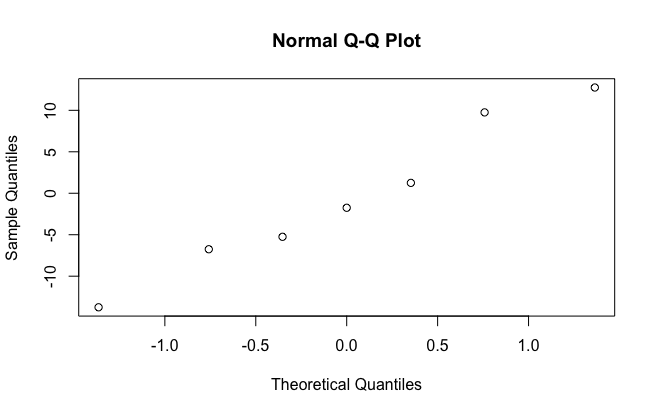
\includegraphics[scale=0.55]{lect18-3-d.png}
\begin{verbatim}
> eff3
      A1       B1       C1   Block1    A1:B1    A1:C1    B1:C1 A1:B1:C1 
    1.25    12.75     9.75    -6.75    -1.75   -13.75    -5.25       NA 
\end{verbatim}

\noindent The qqplot is similar to the one in part a. Since ABC effect or block effect is not significant in first part, significant effects are still A, B, C, AC.

\begin{verbatim}
lm4 <- lm(y~A+B+C+A:C+Block)
summary.aov(lm4)
            Df Sum Sq Mean Sq F value Pr(>F)  
A            1    3.1     3.1   0.102 0.7797  
B            1  325.1   325.1  10.616 0.0827 .
C            1  190.1   190.1   6.208 0.1303  
Block        1   91.1    91.1   2.976 0.2267  
A:C          1  378.1   378.1  12.347 0.0723 .
Residuals    2   61.2    30.6                 
---
\end{verbatim}
\noindent Under the significance level of 0.05, the ANOVA table of blocked model shows no evidence that any of the factors have significant effect. 

\subsection*{e}
\begin{verbatim}
rm(list=ls(all=T))
y <- c(22, 32, 35, 55, 44, 40, 60, 39)
design4 <- gen.factorial(c(2,2,2), varNames = c('A','B','C'))
attach(design4)
AC <- A*C
BC <- B*C
Block <- numeric(8)
for (i in 1:8) {
  if (AC[i] == -1 & BC[i] == -1) {
    Block[i] = 1
  } else if (AC[i] == 1 & BC[i] == -1) {
    Block[i] = 2
  } else if (AC[i] == -1 & BC[i] == 1) {
    Block[i] = 3
  } else {
    Block[i] = 4
  }
}
A <- as.factor(A)
B <- as.factor(B)
C <- as.factor(C)
Block <- as.factor(Block)
lm4 <- lm(y~A*B*C + Block)

summary.aov(lm4)
            Df Sum Sq Mean Sq
A            1    3.1     3.1
B            1  325.1   325.1
C            1  190.1   190.1
Block        3  439.4   146.5
A:B:C        1   91.1    91.1
\end{verbatim}

\noindent Since AC, BC, AB effects are confounded with block effect, these three factors are not shown in ANOVA table. 

\newpage
\subsection*{Lect 19-1}
\subsection*{a}
\begin{verbatim}
rm(list=ls(all=TRUE))
design = gen.factorial(2,4,varNames=c("A","B","C","D"), factors="all")
attach(design)
y = c(45,71,48,65,68,60,80,65,43,100,45,104,75,86,70,96) 
BL = as.factor((c(A) + c(B) + c(C) + c(D)) %% 2 )
A <- as.factor(A)
B <- as.factor(B)
C <- as.factor(C)
D <- as.factor(D)
contr <- as.character("contr.helmert")
lm1 <- lm(y~A*B*C*D*BL, contrasts = list(A=contr,B=contr,C=contr, D=contr, BL=contr))
summary.aov(lm1)
eff <- 2*lm1$coef
eff <- eff[2:16]
ss = summary.aov(lm1) [[1]][,2]

> eff
     A1      B1      C1      D1     BL1   A1:B1   A1:C1   B1:C1   A1:D1   B1:D1 
 21.625   3.125   9.875  14.625  -1.375   0.125 -18.125   2.375  16.625  -0.375 
  C1:D1  A1:BL1  B1:BL1  C1:BL1  D1:BL1 
 -1.125   2.625   1.625  -4.125  -1.875 
> ss
 [1] 1870.5625   39.0625  390.0625  855.5625    7.5625    0.0625 1314.0625   22.5625
 [9] 1105.5625    0.5625    5.0625   27.5625   10.5625   68.0625   14.0625
\end{verbatim}

\subsection*{b}
\noindent The effect and ss values of model that includes block-treatment interaction effects are identical to full model because data is independent to model. All the block-treatment effects are confounded with some kind of treatment interaction. For example, effect ABC is confounded with D-Block effect. 

\subsection*{c}
\noindent Note that ABCD is confounded with Block effect. The effect of interaction between A and Block can be considered as $A \times ABCD$, which by magic is $BCD$. Similarly, effect of ACD is confounded with B and Block for $B \times ABCD = ACD$; effect of ABD is confounded with C and Block; effect of ABC is confounded with D and Block. 

\subsection*{Lect 19-2}
\subsection*{a}
\begin{verbatim}
rm(list=ls(all=TRUE))
design = gen.factorial(2,5,varNames=c("A","B","C","D",'E'), factors="all")
attach(design)
y <- c(7,9,34,55,16,20,40,60,8,10,32,50,18,21,44,61,
       8,12,35,52,15,22,45,65,6,10,30,53,15,20,41,63)
A <- as.factor(A)
B <- as.factor(B)
C <- as.factor(C)
D <- as.factor(D)
E <- as.factor(E)
contr <- as.character("contr.helmert")
lm1 <- lm(y~A*B*C*D*E, contrasts = list(A=contr,B=contr,C=contr, D=contr, E=contr))

summary.aov(lm1)
            Df Sum Sq Mean Sq
A            1   1116    1116
B            1   9214    9214
C            1    751     751
D            1      5       5
E            1      2       2
A:B          1    504     504
A:C          1      2       2
B:C          1      0       0
A:D          1      0       0
B:D          1      4       4
C:D          1      5       5
A:E          1      7       7
B:E          1      3       3
C:E          1      1       1
D:E          1     11      11
A:B:C        1      2       2
A:B:D        1      1       1
A:C:D        1      2       2
B:C:D        1      2       2
A:B:E        1      0       0
A:C:E        1      1       1
B:C:E        1      7       7
A:D:E        1      5       5
B:D:E        1      0       0
C:D:E        1      5       5
A:B:C:D      1      0       0
A:B:C:E      1      0       0
A:B:D:E      1      7       7
A:C:D:E      1      1       1
B:C:D:E      1      7       7
A:B:C:D:E    1      0       0
\end{verbatim}

\subsection*{b}
\begin{verbatim}
rm(list=ls(all=TRUE))
design = gen.factorial(2,5,varNames=c("A","B","C","D",'E'))
attach(design)
y <- c(7,9,34,55,16,20,40,60,8,10,32,50,18,21,44,61,
       8,12,35,52,15,22,45,65,6,10,30,53,15,20,41,63)
ABC = A*B*C 
CDE = C*D*E
BL = numeric(16)
BL[ABC==-1 & CDE==-1] = 1
BL[ABC==+1 & CDE==-1] = 2
BL[ABC==-1 & CDE==+1] = 3
BL[ABC==+1 & CDE==+1] = 4
A <- as.factor(A)
B <- as.factor(B)
C <- as.factor(C)
D <- as.factor(D)
E <- as.factor(E)
BL <- as.factor(BL)
lm2 <- lm(y~A*B*C*D*E+BL)

summary.aov(lm2)
            Df Sum Sq Mean Sq
A            1   1116    1116
B            1   9214    9214
C            1    751     751
D            1      5       5
E            1      2       2
BL           3     14       5
A:B          1    504     504
A:C          1      2       2
B:C          1      0       0
A:D          1      0       0
B:D          1      4       4
C:D          1      5       5
A:E          1      7       7
B:E          1      3       3
C:E          1      1       1
D:E          1     11      11
A:B:D        1      1       1
A:C:D        1      2       2
B:C:D        1      2       2
A:B:E        1      0       0
A:C:E        1      1       1
B:C:E        1      7       7
A:D:E        1      5       5
B:D:E        1      0       0
A:B:C:D      1      0       0
A:B:C:E      1      0       0
A:C:D:E      1      1       1
B:C:D:E      1      7       7
A:B:C:D:E    1      0       0
\end{verbatim}

\subsection*{c}
\noindent The only one difference is Block effect replaced effects of ABC, CDE and ABDE. The degree of Block factor becomes 3, the SS value of Block is equal to sum of all SS's of ABC, CDE and ABDE. This phenomenon shows effects of ABC, CDE and ABDE are confounded with block effect. 

\newpage
\subsection*{Lect 19-5}
\subsection*{a}
\begin{verbatim}
rm(list=ls(all=TRUE))
design = gen.factorial(2,4,varNames=c("A","B","C","D"))
attach(design)
y = c(23,15, 16, 18, 25, 16, 17, 26, 28, 16, 18, 21, 36, 24, 33, 34)
BL <- A*B*C
lm1 <- lm(y~A*B*C*D + BL)

summary.aov(lm1)            Df Sum Sq Mean Sq F value Pr(>F)  
            Df Sum Sq Mean Sq
A            1  42.25   42.25
B            1   0.00    0.00
C            1 196.00  196.00
D            1 182.25  182.25
BL           1   2.25    2.25
A:B          1 196.00  196.00
A:C          1   1.00    1.00
B:C          1  20.25   20.25
A:D          1  12.25   12.25
B:D          1   1.00    1.00
C:D          1  64.00   64.00
A:B:D        1   0.00    0.00
A:C:D        1   4.00    4.00
B:C:D        1   2.25    2.25
A:B:C:D      1   6.25    6.25
\end{verbatim}

\subsection*{b}
\begin{verbatim}
rm(list=ls(all=TRUE))
design = gen.factorial(2,4,varNames=c("A","B","C","D"), factors = 'all')
attach(design)
y = c(23,15, 16, 18, 25, 16, 17, 26, 28, 16, 18, 21, 36, 24, 33, 34)
BL = as.factor((c(A) + c(B) + c(C)) %% 2 )
lm1 <- lm(y~A*B*C*D + BL)

summary.aov(lm1)
            Df Sum Sq Mean Sq
A            1  42.25   42.25
B            1   0.00    0.00
C            1 196.00  196.00
D            1 182.25  182.25
BL           1   2.25    2.25
A:B          1 196.00  196.00
A:C          1   1.00    1.00
B:C          1  20.25   20.25
A:D          1  12.25   12.25
B:D          1   1.00    1.00
C:D          1  64.00   64.00
A:B:D        1   0.00    0.00
A:C:D        1   4.00    4.00
B:C:D        1   2.25    2.25
A:B:C:D      1   6.25    6.25
\end{verbatim}

\subsection*{c}
\begin{verbatim}
BL1 <- as.factor((c(A)+c(B))%%2)
BL2 <- as.factor((c(C)+c(D))%%2)
BL <- numeric(length(y))
BL[BL1==0 & BL2==0] <- 1
BL[BL1==1 & BL2==0] <- 2
BL[BL1==0 & BL2==1] <- 3
BL[BL1==1 & BL2==1] <- 4
BL <- as.factor(BL)
lm2 <- lm(y~A*B*C*D + BL)

summary.aov(lm2)
            Df Sum Sq Mean Sq
A            1  42.25   42.25
B            1   0.00    0.00
C            1 196.00  196.00
D            1 182.25  182.25
BL           3 266.25   88.75
A:C          1   1.00    1.00
B:C          1  20.25   20.25
A:D          1  12.25   12.25
B:D          1   1.00    1.00
A:B:C        1   2.25    2.25
A:B:D        1   0.00    0.00
A:C:D        1   4.00    4.00
B:C:D        1   2.25    2.25
\end{verbatim}

\newpage
\subsection*{Lect 20-2}
\begin{verbatim}
rm(list=ls(all=TRUE))
design <- gen.factorial(2,3,varNames = c('A','B','C'))
attach(design)
y = c(43, 71, 48, 104, 68, 86, 70, 65)
D <- -A*B*C
A <- as.factor(A)
B <- as.factor(B)
C <- as.factor(C)
D <- as.factor(D)
contr = as.character("contr.helmert")
lm1 = lm(y~A*B*C*D, contrasts = list(A=contr,B=contr,C=contr,D=contr))
eff = 2 * lm1$coefficients
eff = eff[2:8]

    A1     B1     C1     D1  A1:B1  A1:C1  B1:C1 
 24.25   4.75   5.75  12.75   1.25 -17.75 -14.25 
\end{verbatim}

\noindent There are seven alias relationships under $2^{4-1}$ design with ABCD=+1. Their effects are shown above.

\subsection*{Lect 20-3}
\subsection*{c}
\begin{verbatim}
rm(list=ls(all=TRUE))
design <- gen.factorial(2,4,varNames = c('A','B','C','E'))
design1 <- rbind(design, design, design)
attach(design1)
rep1 <- c(7.78,8.15,7.50,7.59,7.54,7.69,7.56,7.56,7.50,7.88,7.50,7.63,7.32,7.56,7.18,7.81)
rep2 <- c(7.78,8.18,7.56,7.56,8.00,8.09,7.52,7.81,7.25,7.88,7.56,7.75,7.44,7.69,7.18,7.50)
rep3 <- c(7.81,7.88,7.50,7.75,7.88,8.06,7.44,7.69,7.12,7.44,7.50,7.56,7.44,7.62,7.25,7.59)
y <- c(rep1, rep2, rep3)
D <- A*B*C
A <- as.factor(A)
B <- as.factor(B)
C <- as.factor(C)
D <- as.factor(D)
E <- as.factor(E)
contr = as.character("contr.helmert")
lm1 = lm(y~A*B*C*D*E, contrasts = list(A=contr,B=contr,C=contr,D=contr,E=contr))

summary.aov(lm1)
            Df Sum Sq Mean Sq F value   Pr(>F)    
A            1 0.7033  0.7033  35.888 1.12e-06 ***
B            1 0.3218  0.3218  16.420 0.000302 ***
C            1 0.0295  0.0295   1.506 0.228774    
D            1 0.0999  0.0999   5.099 0.030893 *  
E            1 0.6840  0.6840  34.906 1.42e-06 ***
A:B          1 0.0105  0.0105   0.536 0.469451    
A:C          1 0.0000  0.0000   0.001 0.975515    
B:C          1 0.0063  0.0063   0.322 0.574603    
A:E          1 0.0488  0.0488   2.489 0.124500    
B:E          1 0.2806  0.2806  14.319 0.000640 ***
C:E          1 0.0130  0.0130   0.664 0.421343    
D:E          1 0.0188  0.0188   0.959 0.334662    
A:B:E        1 0.0001  0.0001   0.003 0.959204    
A:C:E        1 0.0046  0.0046   0.235 0.631251    
B:C:E        1 0.0426  0.0426   2.174 0.150128    
Residuals   32 0.6271  0.0196                     
---
\end{verbatim}

\noindent Under the significance level of 0.01, A, B, E, BE factors have significant effect. 

\subsection*{d}
\begin{verbatim}
eff <- as.matrix(2 * lm1$coefficients[-1])
eff <- as.matrix(na.omit(eff))
qqnorm(eff[,1])
abline(median(eff[,1]), 0.08, col=2)
\end{verbatim}

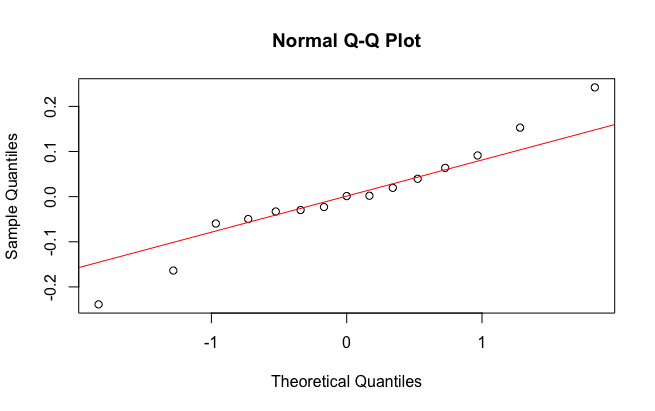
\includegraphics[scale=0.55]{lect20-3-d.png}

\noindent We can perceive from the qqnorm that factors that have highest two effects and lowest two effects are out of linear pattern, indicating they are significant. These four factors are A, B, E, BE.


\end{document}